\chapter{LocText Corpus}\label{chapter:corpus}

\section{Need for a separate corpus}

As mentioned in the previous chapter, the GENIA event corpus or its subset, the BIONLP shared task corpus is not the best corpus that can be used for training a model to extract protein- subcellular location relations. As pointed out previously, following are some of the issues related to the corpus:
\begin{enumerate}
\item Not all the locations found in the GENIA event corpus are subcellular compartments. Some of the locations are the names of cells or tissues in the body.
\item In some mentions of subcellular compartment, the actual mention contains extraneous words in addition to the mention of subcellular compartment. These extraneous words takes away the preciseness of the mention of subcellular compartment.
\item Some localization events does not contain an actual mention of subcellular compartment but the context just points out the clue leading to hypothesis that a localization event may have been mentioned.
\end{enumerate}

To summarize, the GENIA event corpus have some serious concerns and cannot be directly used if we are trying to train a classifier for protein-subcellular compartment relation extraction. There was a need to create a separate corpus dedicated for this task.

\section{LocText}

We annotated a corpus consisting of 100 Medline abstracts. To select the abstracts that contains evidence of subcellular localization of protein, we made a list of PubMed identifiers cited by UniprotKB protein subcellular localization annotations. Out of these list, we chose 100 abstracts randomly. In order to have sufficient taxonomic variation, we made sure that 50 abstracts belonged to human and 25 abstracts belonged each to budding yeast (Saccharomyces cerevisiae) and Arabidopsis (Arabidopsis thaliana).

\section{Corpus annotation process and guidelines}

We started the process of corpus annotation by selection of abstracts and annotation of the corpus was done with the help of tagtog [CITE:TAGTOG]. The corpus was annotated for following things:

\begin{enumerate}
\item Entities
\begin{enumerate}
\item Proteins (includes gene and mRNA mentions)
\item Subcellular compartment
\item Organisms
\end{enumerate}
\item Relations
\begin{enumerate}
\item Protein - Organism
\item Protein - Subcellular compartment
\end{enumerate}
\end{enumerate}

\subsection*{Normalization of entities}

The entities were normalized to a unique identifier in order to have a unique and uniform representation of entities and the relations involving those entities. Protein annotations are normalized to UniprotKB [CITE:UNIPROT KB] identifiers, subcellular localizations are normalized to Gene Ontology (GO) [CITE:NCBI] terms and the organisms are annotated to NCBI Taxonomic [CITE:NCBI] identifiers.

\subsection*{Annotation guidelines}
Out of 100 abstracts, we used 46 abstracts to develop our annotation guidelines. The annotation guidelines along with the full corpus is available at \hyperref[LocText]{https://www.tagtog.net/-corpora/loctext}. Some of the important annotation guidelines we followed are:

\begin{itemize}
\item We annotated the protein names only when these names can be found in UniprotKB [CITE:UNIPROT KB] in context of particular organism.
\item Similarly, we annotated the subcellular compartment if these compartment names can be found in GO ontology [CITE:GO]
\item We annotated organism names if the organism names correspond to rank species, genus or subfamily in NCBI Taxonomy [CITE:NCBI].
\item For all relations (protein-organism \& protein-location), the context is very important and the relations aren't made without sufficient evidence.
\end{itemize}


\begin{figure}[hbtp]
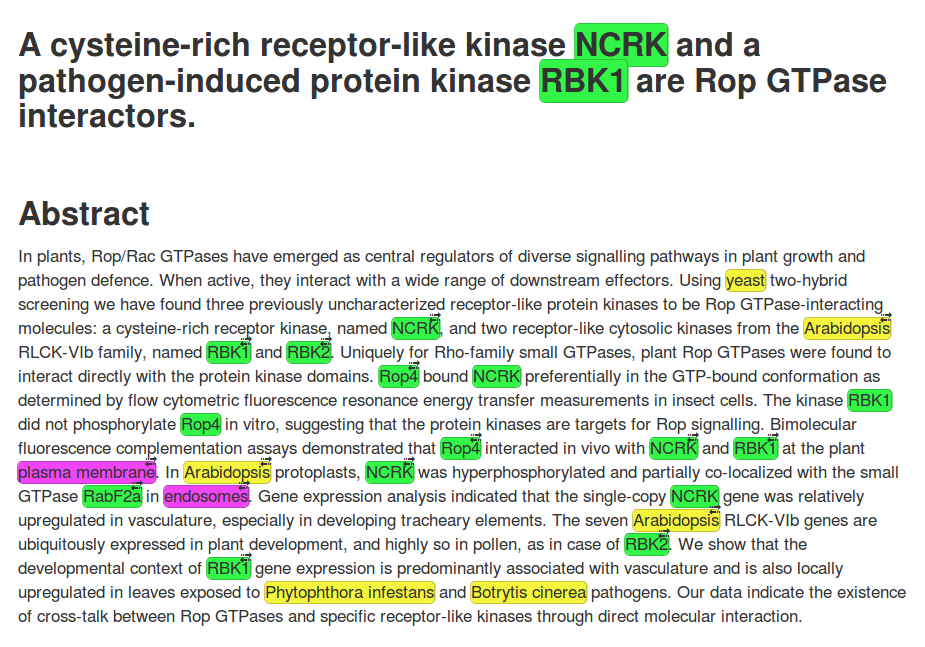
\includegraphics[scale=0.4]{figures/tagtog_screenshot.png}
\caption{Screenshot of an abstract from tagtog annotation tool}\label{tagtogScreenshot}
\end{figure}

Figure \ref{tagtogScreenshot} shows an example abstract annotated in tagtog annotation tool. The proteins, localizations and organisms are highlighted in yellow, green and magenta respectively. The entities which participates in either protein-organism or protein location relation, has a double arrow as an additional marking.

\section{Inter-annotator agreement (IAA)}

As mentioned earlier, 46 abstracts out of 100 were used for developing annotation guidelines and the remaining 54 abstracts were used for calculating Inter-annotator agreement. These 54 abstracts were independently annotated by two annotators based on the annotation guidelines and used for calculation of Inter-annotator agreement denoted by F1 score. The F1 score for entities and relations was calculated by following formula:

$$
F1 = \frac{2*X_{AB}*X_{BA}}{X_{AB}+X_{BA}}
$$

where $X_{ij}$ is the fraction of annotations by annotator i matching those of annotator j.

\subsection*{IAA for entities}

Since, the focus of annotating the corpus was protein subcellular location relation extraction, the IAA was mainly calculated for entities - proteins \& subcellular location and protein-location relation extraction.

We considered two annotations of the same entity to match if they have the exact same start offsets and end offsets. The IAA between two annotators was F1 score of  96\% and 88\% for proteins and location entities respectively. The combined F1 score for entity types was 94\%.

\subsection*{IAA for relations}

we define a protein-subcellular location relation to match between two annotators if annotations of both the protein and location entity match between the annotators, according to the definition above.

The IAA for two annotators was F1 score of 80\% for protein-location relations.

\section{Important insights from the corpus and Publication}

% Explain about the results that you published at the BLAH conference
After annotating the corpus, we could derive some important insights from the corpus. We found out that the database annotations in database such as UniprotKB aren't complete and there is a room for improvement in the annotations in such database.

We published the results [CITE:GOLDBERG ET.AL.] in the symposium at Biomedical Linked Annotation Hackathon (BLAH) [CITE:BLAH]. Since the Biomedical Research Community and Natural Language Processing (NLP) community both undertake the annotations of text with different objectives in mind, we envisioned that creating linked annotations compromising of contributions from both communities would be immensely helpful. 

We started with the annotation of corpus from scratch without actually referring to the annotations present in knowledge-bases like UniProtKB, we found out that we have more annotations for the same set of documents in our corpus compared with UniProtKB.

We compared the protein-location relations present in our corpus with the information already present in the knowledge bases. We divided our annotations in three categories viz. existing, more detailed and novel. Existing annotations are the ones that are present in knowledge-bases already. We define some annotations as more detailed if they provide more information than what is present in the knowledge-bases. In the same way, we define annotations as novel annotations if they are not present in the knowledge bases. The annotations are further subdivided based on whether or not the relationships involve UniprotKB proteins that cite the abstract.

\begin{table}
\centering
\begin{tabular}{|c|c|c|c|c|c|c|}
\hline
\textbf{Category} & \multicolumn{2}{c|}{\textbf{Existing}} & \multicolumn{2}{c|}{\textbf{More detailed}} & \multicolumn{2}{c|}{\textbf{Novel}} \\ 
\hline
\textbf{Citing Protein} & \textbf{Yes} & \textbf{No} & \textbf{Yes} & \textbf{No} & \textbf{Yes} & \textbf{No} \\
\hline
Human & 29 & 15 & 1 & 1 & 14 & 3 \\
Budding Yeast & 22 & 14 & 5 & 3 & 6 & 5 \\
Arabidopsis & 19 & 7 & 5 & 2 & 6 & 7 \\
Other & 2 & 9 & 0 & 0 & 0 & 6 \\
\hline
Subtotal & 72 & 45 & 11 & 6 & 26 & 41 \\
\hline
\textbf{Total} & \multicolumn{2}{c|}{\textbf{117}} & \multicolumn{2}{c|}{\textbf{17}} & \multicolumn{2}{c|}{\textbf{67}} \\ 
 \hline
\end{tabular}
\caption{Comparison of protein subcellular localization annotations in our corpus
and in UniProtKB}\label{tab:novelAnnotation}
\end{table}

% Write about observations from table here
\section{Corpus statistics}

% Put all the numbers with respect to number of entities, relations and their distribution here. Also, put all the nice graphs that you made here

\section{Linked Annotation}

%Write about contribution in BLAH